\documentclass[twocolumn]{article}
\usepackage[utf8]{inputenc}
\usepackage[margin=1in]{geometry}  % 调整页面边距
\usepackage{titling}               % 控制标题位置
\usepackage{booktabs}              % 表格宏包
\usepackage{amssymb}
\usepackage{ctex}                  % 中文支持包
\usepackage{authblk}			   % 多作者
\usepackage{graphicx}
% \usepackage{tabularx}			% 表格宽度
% \usepackage{xeCJK}
\setlength{\droptitle}{-3.0cm}     % 将标题上移3.0厘米

\title{Medical Image Synthesis from CT to PET using Convolutional Neural Network}
\author[1] {Your Name}
\author[1] {Teacher Author}
% \author[1,3]{Third Author}
\affil[1]{University of Fukui, 3-9-1 Bunkyo, Fukui, 910-0019, Japan}
% \affil[2]{Department of Electrical Engineering, University of Y}
% \affil[3]{Research Institute, Company Z}
\date{2024.11.30}

\begin{document}

\twocolumn[
	\maketitle

	\begin{center}
		\begin{abstract}
			This is Abstract chapter.
		\end{abstract}
	\end{center}
	\vspace{0.5cm}  % 调整摘要与正文之间的间距
]

\section{Introduce}
U-Net是一种深度学习架构,它最初是为医学图像分割任务设计的,并且因其出色的性能和高效的结构而在医学图像处理领域广受欢迎。U-Net的架构是对典型的卷积神经网络(CNN)的改进,它具有一个对称的“U”形结构,包含一个收缩(编码)路径和一个扩张(解码)路径。U-Net的一个关键特性是其使用的跳跃连接(或跳过连接),这些连接将收缩路径上的特征图与扩张路径上对应层的特征图相连。这样的设计使得网络能够在上采样过程中利用更精确的空间信息,有助于改善分割边界的精确度,特别是在医学图像中结构的界限清晰非常重要。
U-Net is a deep learning architecture initially designed for medical image segmentation tasks and has become widely popular in the field of medical image processing due to its outstanding performance and efficient structure. The architecture of U-Net is an improvement over the typical convolutional neural network (CNN), featuring a symmetric "U" shape that includes a contracting path (encoder) and an expanding (decoder) path. A key feature of U-Net is its use of skip connections, which connect feature maps from the contracting path to corresponding layers in the expanding path. Such a design allows the network to utilize more precise spatial information during the upsampling process, which is crucial for enhancing the accuracy of segmentation boundaries, especially where the delineation of structures in medical images is critically important.


\section{Related Works}
Since its introduction by Olaf and colleagues \cite{navab_u-net_2015}, U-Net has been widely used due to its structural advantages and excellent performance in applications such as image denoising \cite{armanious_medgan_2020}, medical image registration \cite{singh_automated_2023}, and attenuation correction \cite{liu_deep_2018}. It is also applied to various other image segmentation tasks including lesion segmentation \cite{du_medical_2020} and face image restoration \cite{zeng_swin-casunet_2022}.

In experiments using U-Net or other image segmentation and reconstruction models, it is crucial to evaluate the accuracy, reliability, and effectiveness of the model's performance. Various quantitative metrics commonly used in U-Net related experiments help researchers and developers understand the model's performance in specific tasks.

The Structural Similarity Index Measure (SSIM) is a complex metric used to measure the structural similarity between two images. It considers aspects such as luminance, contrast, and structural information of the images. The SSIM value ranges from -1 to 1, where 1 indicates perfect similarity. This metric is particularly useful in medical image segmentation as it provides a detailed reflection of the visual and structural quality of the images.

The Multi-Scale Structural Similarity Index Measure (MS-SSIM) is an extension of SSIM that evaluates image similarity across multiple scales, offering a more comprehensive assessment of image quality. This is especially useful when dealing with medical images that vary significantly in resolution.

Visual Information Fidelity (VIF) is a metric for image quality assessment based on natural scene statistics and human visual system characteristics. VIF attempts to simulate the human eye's perception of image quality and considers the degree of information loss during the image transmission process. VIF operates from an information-theoretic perspective, comparing the preservation of information between the original and distorted images.

Peak Signal-to-Noise Ratio (PSNR) is another widely used metric to measure the quality of image reconstruction. It is employed in fields like image and video compression and other forms of signal processing to assess the quality of an image reconstruction or compression by comparing the similarity between the original and processed images.

Mean Squared Error (MSE) is one of the most commonly used metrics to evaluate the quality of an image reconstruction. It calculates the average of the squares of the pixel intensity differences between the reconstructed image and the original image. The lower the MSE value, the smaller the error in image reconstruction and the higher the quality.

This study will utilize the standard U-Net model to perform cross-modality conversion tasks from CT to PET images and demonstrate the model's performance using the above metrics.

\section{Method}
U-Net's architecture is designed symmetrically, with a contracting path (Encoder) to capture context and a symmetric expanding path (Decoder) that enables precise localization. This study aims to construct a standard U-Net, a convolutional neural network, to develop a cross-modality medical image converter from CT to PET images. The model will be optimized using a specific loss function suitable for this type of image conversion task.

\subsection{Encoder}
The encoder follows the typical architecture of a convolutional network. It consists of repeated application of two $3\times3$ convolutions, each followed by a rectified linear unit (ReLU) and a $2\times2$ max pooling operation with stride 2 for downsampling. At each downsampling step, the number of feature channels is doubled. The convolution operation in U-Net can be described by the following equation:
\[
I' = \sum_{i,j} (I * K)(i,j) + b
\]
where \(I\) represents the input image, \(K\) is the convolution kernel, \(b\) is the bias, and \(I'\) is the output feature map.

Max pooling in the encoder is used to reduce the spatial dimensions of the input feature maps:
\[
P(x,y) = \max(I(x + i, y + j))
\]
where \(P(x,y)\) is the pooled output, and \(I(x + i, y + j)\) represents the input in the neighborhood around location \((x, y)\).



\subsection{Decoder}
The decoder includes a series of upsampling and convolution operations. Each step in the expanding path includes an upsampling of the feature map followed by a $2\times2$ convolution that halves the number of feature channels, a concatenation with the correspondingly cropped feature map from the contracting path, and two $3\times3$ convolutions, each followed by a ReLU. Up sampling in the expanding path uses transposed convolutions to increase the size of the feature map:
\[
U = K^T * I
\]
where \(K^T\) is the transposed convolution kernel and \(U\) is the upsampled output.


\section{Experiments}
本研究将U-Net用于医学图像跨模态转换任务,旨在构建一个U-Net,输入一个CT图像,将其转换为对应的PET图像。In this study, the Lung PET or CT scan data\cite{li_large-scale_2020} were powered by the National Cancer Institute Cancer Imagine Program (CIP).该数据集涵盖了355名受试者的肺部扫描图像,共计251135张扫描图。这些数据主要收集自2009年至2011年间,包括了每位受试者的性别、年龄、体重、吸烟史及癌症诊断分类信息。数据集中的所有扫描数据均以DICOM格式存储。本研究利用Windows操作系统中的MicroDicom软件处理这251135份扫描数据。数据集中的受试者按癌症类型进行标记:类型A代表腺癌,类型B代表小细胞癌,类型E代表大细胞癌,类型G代表鳞状细胞癌。在该数据集中,并非所有受试者的资料均包含PET扫描与CT扫描。因此,本研究筛选仅使用了被诊断为小细胞癌(B类)的38名受试者的扫描数据,这些数据包括PET扫描、多种CT扫描以及融合增强后的扫描图像。在这38名受试者中,仅有9人同时拥有PET扫描与CT扫描的数据,共计12930张扫描图像。通过精确筛选,将切片位置误差不超过0.2mm的PET/CT扫描定义为配对扫描数据,最终获取928张扫描图像。这464对PET/CT肺部扫描数据图像,供本研究使用。本研究实验中的数据划分情况如表\ref{tab:dataset_partition_1}.

% 插入三线表
\begin{table}[h]
	\centering
	\caption{Dataset Partition of Experiment}
	\label{tab:dataset_partition_1}
	\begin{tabular}{cccc}
		\toprule
		Params count & Test  & Train & Total  \\
		\midrule
		Lung PET/CT Pair & 64   & 400 & 464 \\
		Total Images    & 128   & 800 & 928 \\
		\bottomrule
	\end{tabular}
\end{table}

本研究构建了一个标准U-Net模型,模型的参数规模约5千万。我们将得到的464对PET/CT肺部扫描数据导出为256×256像素的RGB格式的PNG图像,自行划分为训练数据集和测试数据集。数据集具体划分情况如下表


本实验采用标准U-Net模型以计算机断层扫描(CT)图像为输入,合成正电子发射断层扫描(PET)图像。仅使用MSE损失作为损失函数,(使用L2损失的优势)。模型优化器采用Adam优化器,学习率(lr)设定为0.001。这一相对较低的学习率有助于模型在训练过程中稳定地逼近全局最优解。最好的实验结果如表\ref{exp_result}所示。

\begin{table}[h]
	\centering
	\caption{SSIM,PSNR,MSE Results of Experiment}
	\label{tab:exp_result}
	\begin{tabular}{cccc}
		\toprule
		Best Result & SSIM & PSNR & MSE  \\
		\midrule
		Train & 0.7854 & 17.6365 & 0.0237 \\
		Test  & 0.7943 & 17.8871 & 0.0235 \\
		\bottomrule
	\end{tabular}
\end{table}

模型在训练集和测试集上的性能表现相似,没有出现过拟合现象。

为了增强模型的泛化能力并缓解过拟合问题,我们采用L2正则化,权重衰减(weight decay)参数设置为0.001。实验过程中记录了200个训练周期的数据,包括Loss,ssim,multi-scale ssim,vif,psnr,mse,每个Epoch训练完成后进行一次测试,训练时的损失值\ref{fig:loss_train},训练和测试时的SSIM\ref{fig:ssim},MS-SSIM\ref{fig:msssim},VIF\ref{fig:vif},PSNR\ref{fig:psnr},MSE\ref{fig:mse}指标的变化情况如相应表格所示。模型在训练集和测试集中均取得不错的性能表现。

% TODO: \usepackage{graphicx} required
\begin{figure}[h]
    \centering
    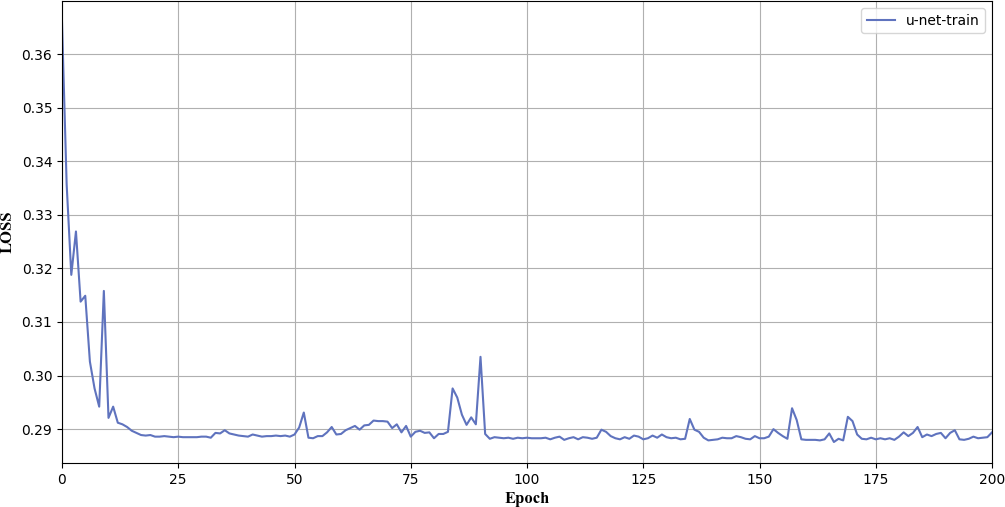
\includegraphics[width=1.0\linewidth]{u-net/LOSS}
    \caption[loss_train]{Loss Line Figure of All Epoch in Train Process}
    \label{fig:loss_train}
\end{figure}

在最初的几个训练周期中,损失值迅速下降,从约0.36降至接近0.29。这表明模型在初期对训练数据的拟合效果迅速提升,学习过程在这一阶段是非常有效的。在快速下降后,损失值趋于稳定,在0.29附近波动。这种趋势表明模型可能已经达到了其训练的稳定状态,进一步的学习导致的性能提升有限。尽管损失值相对稳定,但在某些周期(如50、100和175周期左右)仍有小幅的波动。这些波动可能是由于训练过程中的随机性因素,如批处理数据的随机选择、学习率调整或外部干扰等。整体而言,损失值在200个训练周期内保持相对低且稳定,说明模型具有一定的泛化能力,并在整个训练过程中维持了较好的稳定性。

\begin{figure}[h]
    \centering
    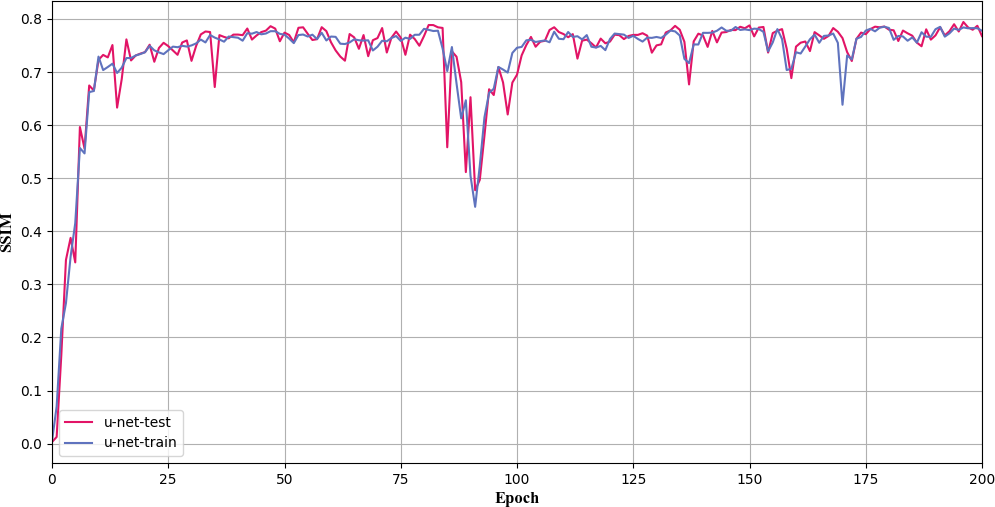
\includegraphics[width=1.0\linewidth]{u-net/SSIM}
    \caption[ssim]{SSIM Line Figure of All Epoch in Train and Test Process}
    \label{fig:ssim}
\end{figure}

图中显示,SSIM值在训练的最初阶段(前25个Epoch)迅速上升,从近0提高到约0.6以上。这表明U-Net模型迅速学习了CT到PET图像之间的映射关系,初期学习效果显著。在经历了快速增长之后,SSIM值在训练和测试集上均趋于稳定,主要在0.7附近波动。这表明模型在继续训练过程中维持了较高的图像重建质量。在整个训练过程中,训练集的SSIM通常高于测试集,这可能是轻微的过拟合迹象,表明模型可能对训练数据过度优化,而对未见的测试数据泛化能力稍弱。

\begin{figure}[h]
    \centering
    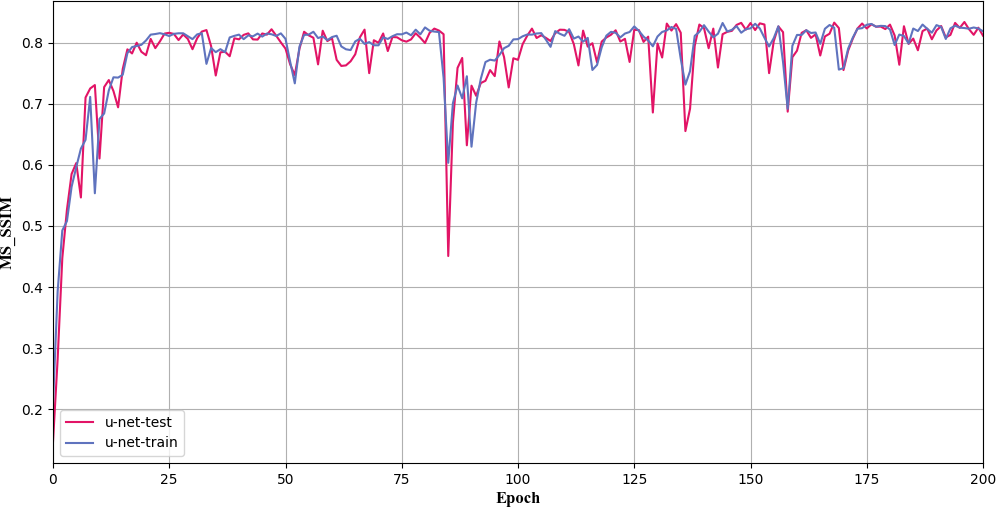
\includegraphics[width=1.0\linewidth]{u-net/MS_SSIM}
    \caption[msssim]{MS-SSIM Line Figure of All Epoch in Train and Test Process}
    \label{fig:msssim}
\end{figure}

图中显示,无论是训练还是测试数据集,MS-SSIM值在最初几个Epoch内迅速提升。这表明模型在学习初期就有效地捕捉到了从CT到PET图像转换的关键特征和结构信息。在初始快速提升之后,MS-SSIM值进入一个较为稳定的波动阶段,这在训练和测试数据上都有体现。训练数据的MS-SSIM值略高于测试数据,这在机器学习模型中是常见的现象,可能表明存在轻微的过拟合。在约50个Epoch之后,尽管有些波动,但MS-SSIM值整体保持在较高水平,特别是在0.7以上,这说明模型对图像的结构相似性有很好的捕捉能力。测试集上的MS-SSIM值整体略低于训练集,但两者之间的差距较小,说明模型在未见数据上也有良好的表现。

\begin{figure}[h]
    \centering
    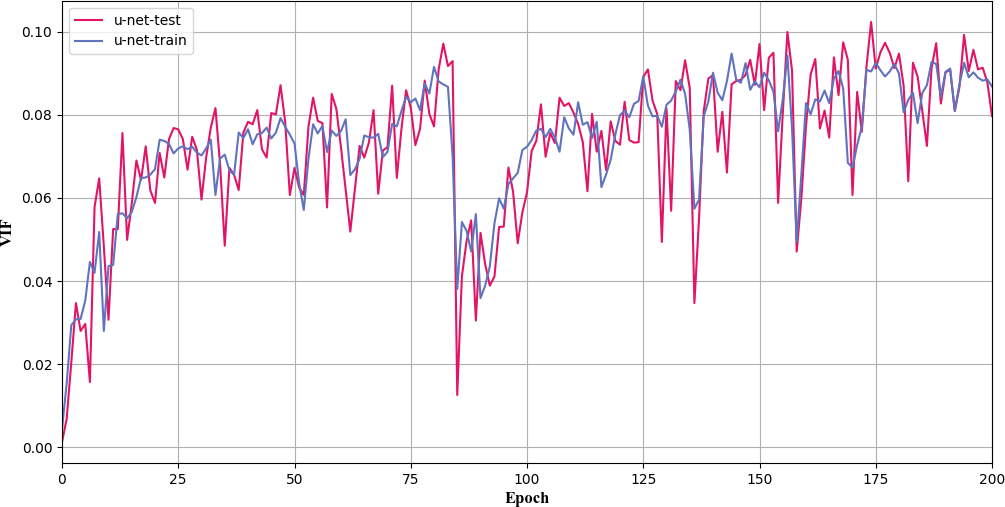
\includegraphics[width=1.0\linewidth]{u-net/VIF}
    \caption[vif]{VIF Line Figure of All Epoch in Train and Test Process}
    \label{fig:vif}
\end{figure}

在最初的几个Epoch中,VIF指数快速上升,这表明模型迅速适应了数据,开始有效地从CT图像中重建出PET图像的视觉信息。这是一个积极的迹象,显示出模型在学习和捕捉两种图像类型间转换的关键特征方面的效率。在经历初期增长后,VIF值在训练和测试过程中表现出相似的波动模式,这可能是因为模型在处理不同的数据批次时遇到的变化性问题。图中显示在某些Epochs,如75、100和175,训练和测试曲线都有显著的峰值和谷值,这可能与数据集中的某些特别的图像或噪声较多的图像有关。训练和测试的VIF曲线在整个实验过程中大致趋同,尽管测试曲线通常略低于训练曲线。这种趋势表明模型对未见数据具有一定程度的泛化能力,尽管这种能力可能存在局限。

\begin{figure}[h]
    \centering
    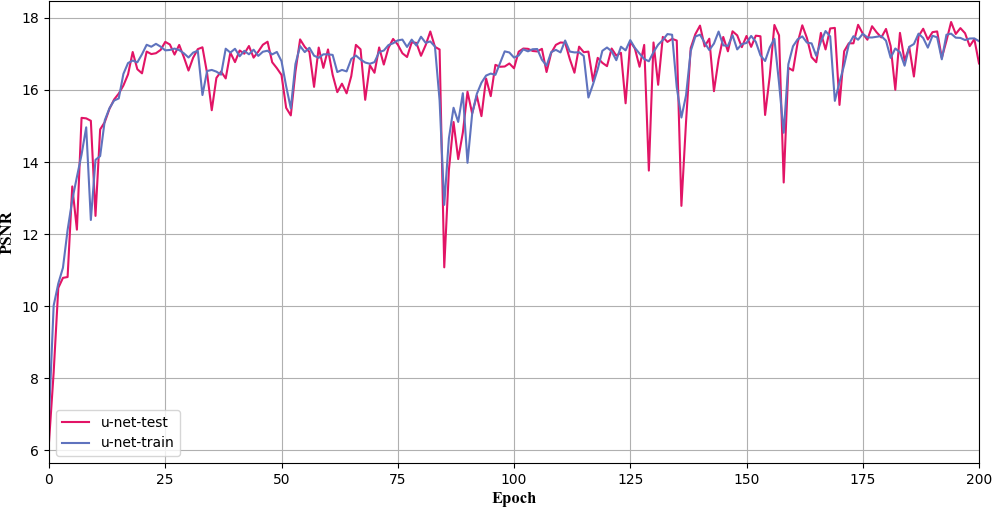
\includegraphics[width=1.0\linewidth]{u-net/PSNR}
    \caption[psnr]{PSNR Line Figure of All Epoch in Train and Test Process}
    \label{fig:psnr}
\end{figure}

图中显示,无论是训练(蓝色线)还是测试(红色线)集,PSNR值在初始的几个Epoch内迅速提升,这表明模型很快就开始有效地从CT图像重建出PET图像。初期的快速提升可能与模型参数的快速调整有关,使得重建的图像质量显著提高。在初期增长之后,PSNR值趋于稳定,但在训练和测试过程中均出现了多次显著的波动。这种波动可能反映了模型在遇到数据中的困难样本时的性能变化,或者是学习过程中的优化算法(如学习率调整等)导致的。尽管存在波动,PSNR在大多数时间内保持在相对较高的水平,表明模型能较好地重建PET图像,且在训练和测试期间展示了一致的性能。训练集和测试集的PSNR曲线十分接近,说明模型对未见数据具有良好的泛化能力。尽管如此,测试集的曲线在某些点下降到低于训练集,这可能是由于测试集中某些特别的图像样本比训练集中的样本更具挑战性。

\begin{figure}[h]
    \centering
    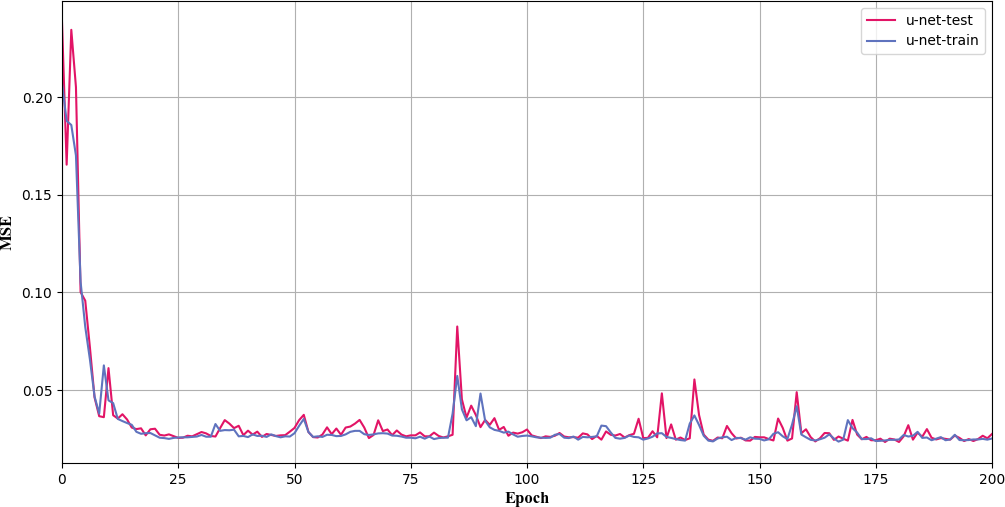
\includegraphics[width=1.0\linewidth]{u-net/MSE}
    \caption[mse]{MSE Line Figure of All Epoch in Train and Test Process}
    \label{fig:mse}
\end{figure}

从图中可以看到,在最初几个Epoch内,训练集和测试集上的MSE都迅速下降,从初始的0.20左右降至约0.05以下。这表明模型在学习初期对从CT到PET的图像转换进行了迅速有效的适应,学习速度较快。
在MSE快速下降之后,训练和测试MSE趋于稳定,但仍有几个明显的峰值,特别是在大约125和175个Epoch时。这些峰值可能反映了模型在处理某些特定的数据批次或异常图像样本时的性能波动。除了偶尔的峰值外,MSE在大多数时间内保持在较低的水平,显示了模型在整个训练和测试过程中的相对稳定性。这表明模型在大部分情况下能够可靠地进行图像重建。训练集和测试集的MSE曲线非常接近,这表明模型对未见数据具有良好的泛化能力。这种接近的趋势还表明模型没有显著的过拟合问题。

\section{Conclusion}
本研究深入探讨了U-Net的发展历史、技术原理及其实际应用,并在医学图像分类任务中进行了实证研究。实验结果表明U-Net模型在CT到PET的图像转换任务中表现出了较高的效率和稳定性。通过进一步的调整和优化,有望在未来应用中实现更佳的性能。

\section*{Acknowledage}
谨此对National Cancer Institute Cancer Image Program表示诚挚的谢意。该机构慷慨地在互联网上公开并授权使用其高质量医疗图像数据集,为本研究的顺利开展提供了不可或缺的资源支持。

\bibliographystyle{unsrt}
\bibliography{unet_ref}

\end{document}
